\documentclass[tikz, border=10pt]{standalone}
\usetikzlibrary{shapes.geometric, arrows.meta, positioning, calc}

\begin{document}

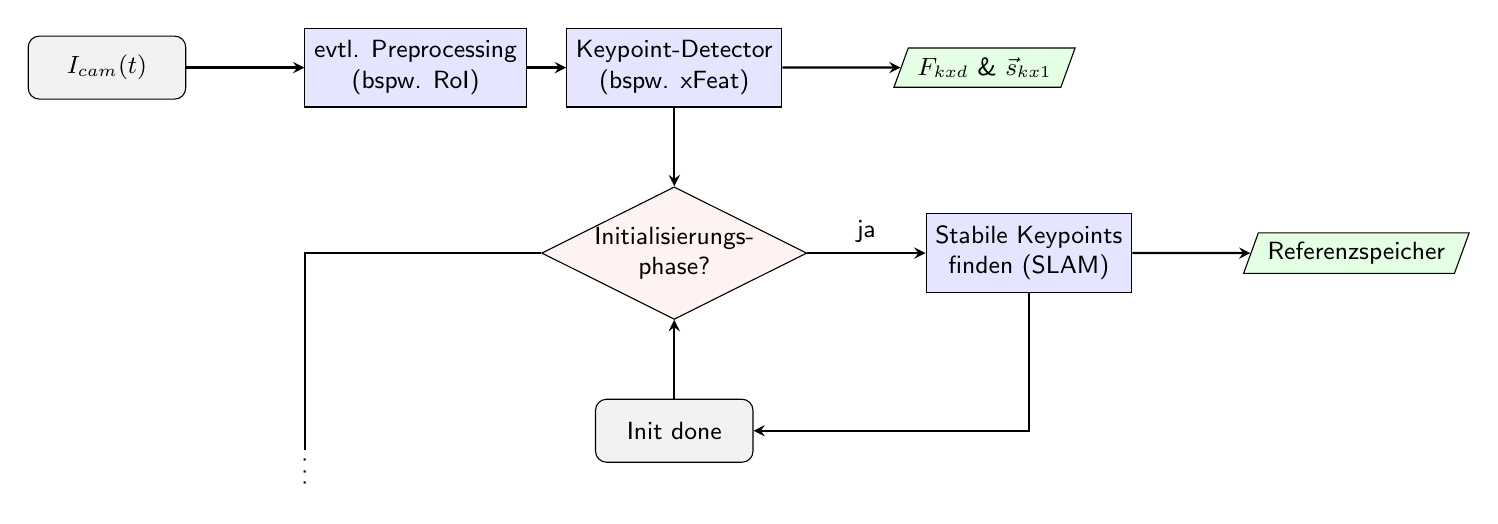
\begin{tikzpicture}[
    node distance=1cm and 1.5cm,
    font=\sffamily\small,
    % Styles für die verschiedenen Formen
    startstop/.style={rectangle, rounded corners, draw, fill=gray!10, minimum width=2cm, minimum height=0.8cm, align=center},
    process/.style={rectangle, draw, fill=blue!10, minimum width=2.5cm, minimum height=1cm, align=center},
    decision/.style={diamond, draw, fill=red!5, aspect=2, inner sep=0pt, minimum width=3cm, align=center},
    data/.style={trapezium, draw, trapezium left angle=70, trapezium right angle=110, fill=green!10, align=center},
    storage/.style={parallelogram, draw, fill=orange!10, minimum width=2cm, align=center},
    % subprocess/.style={circle, draw, fill=yellow!20, minimum size=1.5cm, align=center};
    arrow/.style={thick, ->, >=stealth},
    line/.style={thick, -, >=stealth}
]

% --- Ebene 1: Input & Keypoints ---
\node (input) [startstop] {$I_{cam}(t)$};
\node (preproc) [process, right=of input] {evtl. Preprocessing\\(bspw. RoI)};
\node (keypoint) [process, right=0.5cm of preproc] {Keypoint-Detector\\(bspw. xFeat)};
\node (feat_vec) [data, right=of keypoint] {$F_{kxd}$ \& $\vec{s}_{kx1}$};

% --- Ebene 2: Initialisierung vs. Tracking ---
\node (init_check) [decision, below=of keypoint] {Initialisierungs-\\phase?};
\node (stable_kp) [process, right=of init_check] {Stabile Keypoints\\finden (SLAM)};
\node (ref_store) [data, right=of stable_kp] {Referenzspeicher};
\node (init_done) [startstop, below=of init_check] {Init done};


% --- Verbindungen ---
\draw [arrow] (input) -- (preproc);
\draw [arrow] (preproc) -- (keypoint);
\draw [arrow] (keypoint) -- (feat_vec);
\draw [arrow] (keypoint) -- (init_check);

\draw [arrow] (init_check) -- node[anchor=south] {ja} (stable_kp);
\draw [arrow] (stable_kp) -- (ref_store);
\draw [arrow] (stable_kp) |- (init_done);
\draw [arrow] (init_done) -- (init_check);
\draw [line] (init_check.west) -- ++(-3,0) |- ++(0,-2.5) node[below, anchor=east, rotate=90, xshift=0.1cm] {\dots};

\end{tikzpicture}
\end{document}